\section{Data Entity Design}
Entity classes define a data object which can be persisted to a database via JPA. They have data fields and accessor methods only. They do not implement any logic, but have annotations which instruct the Java Persistence API and ReST API on how to handle individual fields of data.
\\
\begin{center}
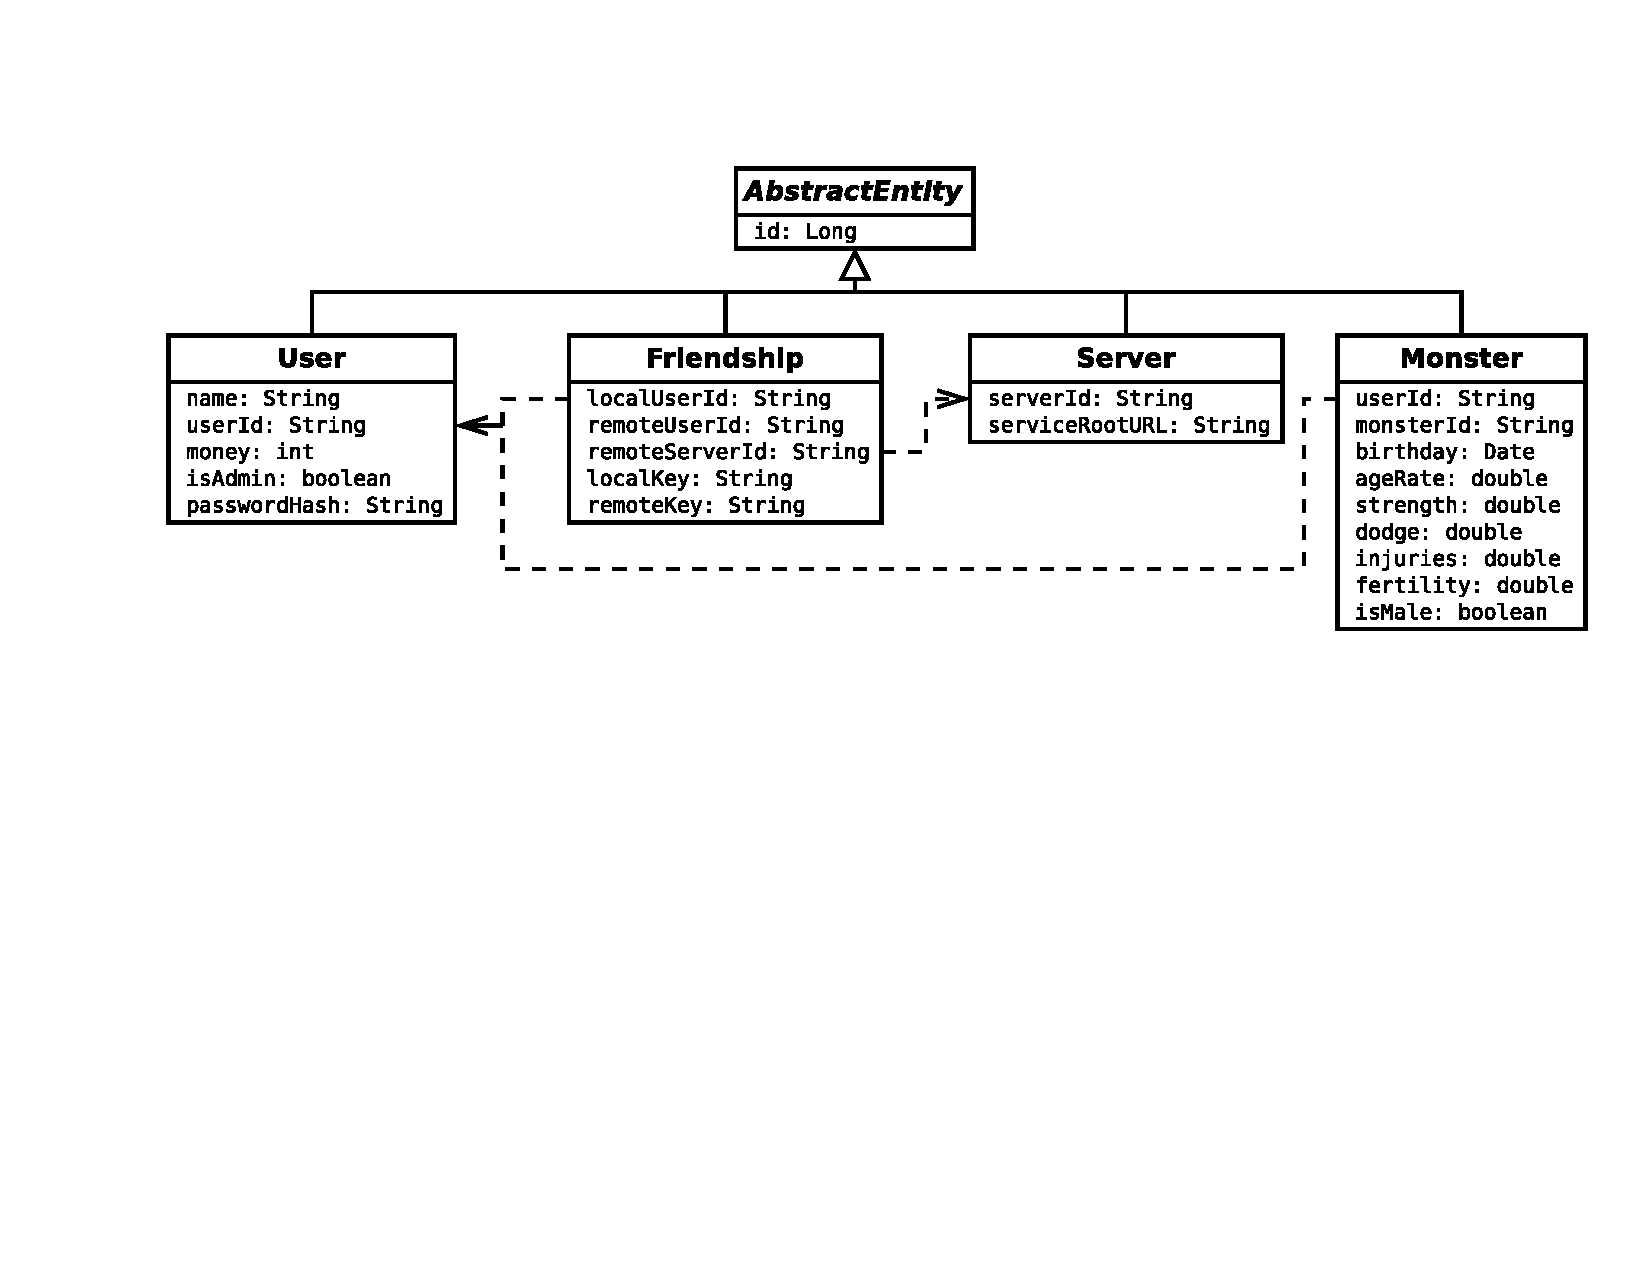
\includegraphics[width=\textwidth]{img/entitydiagram.pdf} 
\end{center}

This diagram describes the entity model design of the application. Each attribute which refers to another entity type is shown as a dashed line \textit{(see Relationships below)}.

\paragraph{Persistence}
Instances of entities (objects) are handled via the Entity Manager, which is provided by JPA and the Glassfish server. JPA talks to the database, and knows how to retrieve and persist these objects correctly. JPA automatically creates SQL tables based on the structure of an entity, eliminating the requirement for database design, as it can all be done by designing entities in Java. To simplify the process of retrieving and persisting Entity objects through JPA, Facade classes should be used instead of acquiring and interfacing with the Entity Manager directly, as described in Section 3.

\paragraph{Manipulation}
Entity objects can be created from scratch by simple instantiating an entity class, or an existing object can be retrieved from the database by using the entity's corresponding Facade.
\\Once you have an entity object instance, it's data can be directly manipulated through it's accessor methods.
\\The entity object can then be persisted to the database (as a new entity or updating the existing one) by passing it to the appropriate method in the Facade.

\paragraph{Relationships}
Relationships in the entity model are not hard coded in. That is, references to other types of entities are refereed to by an identifier attribute. For example, Friendship has a \textbf{localUserId} attribute, which should refer to a \textbf{User} entity via it's \textbf{userId} attribute.
\\The reason that entities do not have formal relationships (one-to-many, one-to-one etc) is that these entities need to be serialised and shared across ReST. By only having a referring ID as a reference to other entity types, this makes the entities more portable. Referenced entity objects can be obtained using lookup methods in the entity's correlating facade.

\paragraph{Annotations}
Entity classes make use of annotations, which describe how the data fields and accessors in the class should be used by JPA and the JSON serialiser for use in REST. JSON annotations are described in \textbf{AbstractEntity}.\\
One of the JPA annotations is \texttt{@NamedQuery}, which defines a JPQL (Java Persistence Query Language) query for this entity class. JPQL is similar to SQL. These are used by Facades to find and manipulate entities stored in the database. Multiple \texttt{@NamedQuery} annotations are contained in a \texttt{@NamedQueries} annotation. \\
Other JPA annotations specify whether fields are optional and whether their values should be unique in the database table, examples of which are in the interface descriptions below.

\clearpage
\subsection{AbstractEntity} An abstract entity which all entity classes should inherit and extend. AbstractEntity does not get persisted to the database, and has no use as a data object in the application.
\\The \textbf{id} attribute is an automatically generated, unique, long integer for uniquely identifying entity objects from the database. As each entity class inherits this attribute, it can be used to uniquely identity an entity object internally (e.g. in a JSP form), but is not much use beyond that.
\\The \texttt{@JsonAutoDetect(JsonMethod.NONE)} annotation instructs the JSON serialiser to ignore all properties by default. For properties to be serialised, they must be explicitly annotated to be so, or have the \texttt{@JsonAutoDetect} annotation overridden in a subclass, and instead choose properties to \textit{not} be serialised.
\begin{small}\begin{verbatim}
@MappedSuperclass
@JsonAutoDetect(JsonMethod.NONE)
public abstract class AbstractEntity implements Serializable {

    @Id
    @GeneratedValue(strategy = GenerationType.AUTO)
    @Basic(optional = false)
    private Long id;
    
    public Long getId();

}
\end{verbatim}\end{small}

\subsection{Server} References to remote servers. Contains their name, which should be unique across all compatible servers, and the URL from which REST services can be accessed.
\begin{small}\begin{verbatim}
@Entity
...
public class Server extends AbstractEntity {
    
    /* Fields */
    
    /* The unique identifier of the server.
     * This is what the server has decided to be named, and should be unique among all other servers.
     * Required */
    @Basic(optional = false)
    @Column(unique = true)
    private String name;
    
    /* The base URL of REST services of the server.
     * Requires a full URI description including the protocol.
     * For example "http://www.myserver.com:8080/myapp/webresources" */
    @Basic(optional = false)
    private String serviceRootURL;
    
    /* Constructors */
    
    public Server();
    public Server(String name, String serviceRootURL);
    
    /* Accessors */

    public String getName();
    public void setName(String name);
    public String getServiceRootURL();
    public void setServiceRootURL(String serviceRootURL);
}

\end{verbatim}\end{small}

\clearpage
\subsection{User}
Describes a user of the application or a compatible application with a different implementation. It has properties such as the user's name, their unique user ID, a hash of their password used to logon, and how much money the user has. This entity can be used to both represent 'local' users, that is users who have registered with and logon to this server, and remote users on other servers via REST, where not all attributes will have data (e.g. no password).
\\User entities which represent remote users should not be persisted to the database.
\begin{small}\begin{verbatim}
@Entity
...
public class User extends AbstractEntity {
    
    /* Fields */
    
    /* A unique identifier for the user. This should not change after the user is created.
     * Will be used by other entities to refer to this object.
     * Can be a short string like "jab41" or an email address for example. */
    @Basic(optional = false)
    private String name;
    
    /* The users real name. This is not a unique identifier. Not required.
     * Used as a more friendly representation of the user to others. */
    @Basic(optional = false)
    @Column(unique = true)
    private String userId;
    
    /* The amount of money the user has as an integer. Required to be at least 0. */
    @Basic(optional = false)
    private Integer money;
    
    /* A boolean indicating whether the user as administrative privileges,
     * and thus whether administrative facilities will be available to the user when logged on.
     * Required for local users only. Should default to false. Not exposed to REST. */
    @Basic(optional = false)
    private Boolean isAdmin;
    
    /* A SHA-1 hash of the user's password.
     * Plain-text passwords are never stored on the database, or used within the application.
     * Instead, passwords should be hashed by a one-way function (SHA-1).
     * To validate a password, hashes can simply be compared.
     * Required for local users only. Not exposed to REST. */
    private String password;
    
    /* Constructors */
    
    public User();
    public User(String userId, String name);
    public User(String userId, String name, String password);
    public User(String userId, String name, String password, boolean isAdmin);
    
    /* Accessors */
    
    @JsonProperty
    public String getName();
    public void setName(String name);
    @JsonProperty
    public String getUserID();
    public void setUserID(String userId);
    public Boolean getIsAdmin();
    public void setIsAdmin(Boolean isAdmin);
    public void setPassword(String password);
    public String getPasswordHash();
}
\end{verbatim}\end{small}

\clearpage
\subsection{Friendship}
Defines a 'friendship' between users. The entity references both a local user and another user, which can be local or remote. Users are referred to by the \textbf{UserID} attribute as defined in the \textbf{User} entity.
\\The server which the remote user is located on is specified by referring to a \textbf{Server} entity via the \textbf{remoteServerId} attribute.
\\Keys are used for handshake authentication between servers, so that friendships cant be manually 'forced'. The key exchange happens only when each user accepts the friend request, and those keys are used to validate operations that only friends can do.
\begin{small}\begin{verbatim}
@Entity
...
@JsonAutoDetect(JsonMethod.GETTER)
public class Friendship extends AbstractEntity {
    /* Fields */
    
    /* The userId of the local user of this friendship. Required. */
    @Basic(optional = false)
    private String localUserId;
    
    /* The userId of the user on the remote server. Required. */
    @Basic(optional = false)
    private String remoteUserId;
    
    /* The serverId of the server which hosts the remote user. Required. */
    @Basic(optional = false)
    private String remoteServerId;
    
    /* The key which the remote server requires to interact with the local user.
     * Not null only when the local user has accepted the friend request. */
    @Column(unique = true)
    private String localKey;
    
    /* The key which this server requires to interact with the remote user on the remote server.
     * Not null only when the remote user has accepted the friend request. */
    private String remoteKey;
    
    /* Constructors */
    
    public Friendship();
    public Friendship(String localUserId, String remoteUserId, String remoteServerId, String localKey,
                      String remoteKey);
    /* Methods */
    
    /* Is a local request (i.e. has been sent from a remote server) */
    public boolean isLocalRequest();
    
    /* Is a remote request (i.e. has been sent to a remote server) */
    public boolean isRemoteRequest();
    
    /* Is an accepted request (has both local and remote keys) */
    public boolean isAccepted();
    
    /* Accessors */

    public String getLocalUserId();
    public void setLocalUserId(String localUserId);
    public String getRemoteUserId();
    public void setRemoteUserId(String remoteUserId);
    public String getRemoteServerId();
    public void setRemoteServerId(String remoteServerId);
    public String getLocalKey();
    public void setLocalKey(String localKey);
    public String getRemoteKey();
    public void setRemoteKey(String remoteKey);   
}
\end{verbatim}\end{small}

\clearpage
\subsection{Monster} The Monster class acts as a hold for the Monster data. The data will be as static as possible, to prevent the need for multiple reads/writes from/to the database. The data stored in this class is: its time of birth (or birthday); its age rate (ageRate); its strength; its dodge-chance (dodge); any health deducted due to battle (injuries); its fertility; and finally, its gender.

\begin{small}\begin{verbatim}
@Entity
...
public class Monster extends AbstractEntity {
    
    /* Attributes */
    @Basic(optional=false)
    private String userId;
    
    @Basic(optional=false)
    @Temporal(TemporalType.DATE)
    private Date birthday;
    
    @Basic(optional=false)
    private double ageRate;
    
    @Basic(optional=false)
    private double strength;
    
    @Basic(optional=false)
    private double dodge;
    
    @Basic(optional=false)
    private double injuries;
    
    @Basic(optional=false)
    private double fertility;
    
    @Basic(optional=false)
    private boolean isMale;
    
    
    /* Constructors */
    public Monster();
    public Monster(double ar, double d, double s, double f, boolean m);
    
    /* Getters and setters */
    
    public String getUserID();
    public void setUserID(String id);
    public Date getBirthday();
    public void setBirthday(Date b);
    public double getAgeRate();
    public void setAgeRate(double ar);
    public double getStrength();
    public void setStrength(double s);
    public double getDodge();
    public void setDodge(double d);
    public double getInjuries();
    public void setInjuries(double i);
    public double getFertility();
    public void setFertility(double f);
    public boolean getIsMale();
    public void setIsMale(boolean m);
}
\end{verbatim}\end{small}
